\begin{figure}
  \begin{tabular}{ccc}
    \begin{minipage}{0.33\hsize}
      \includegraphics[width=4.3cm]{../pic/Run78/KN_ana_NC170_2sigma/KNpi_MM_0.eps}
    \end{minipage}
    \begin{minipage}{0.33\hsize}
      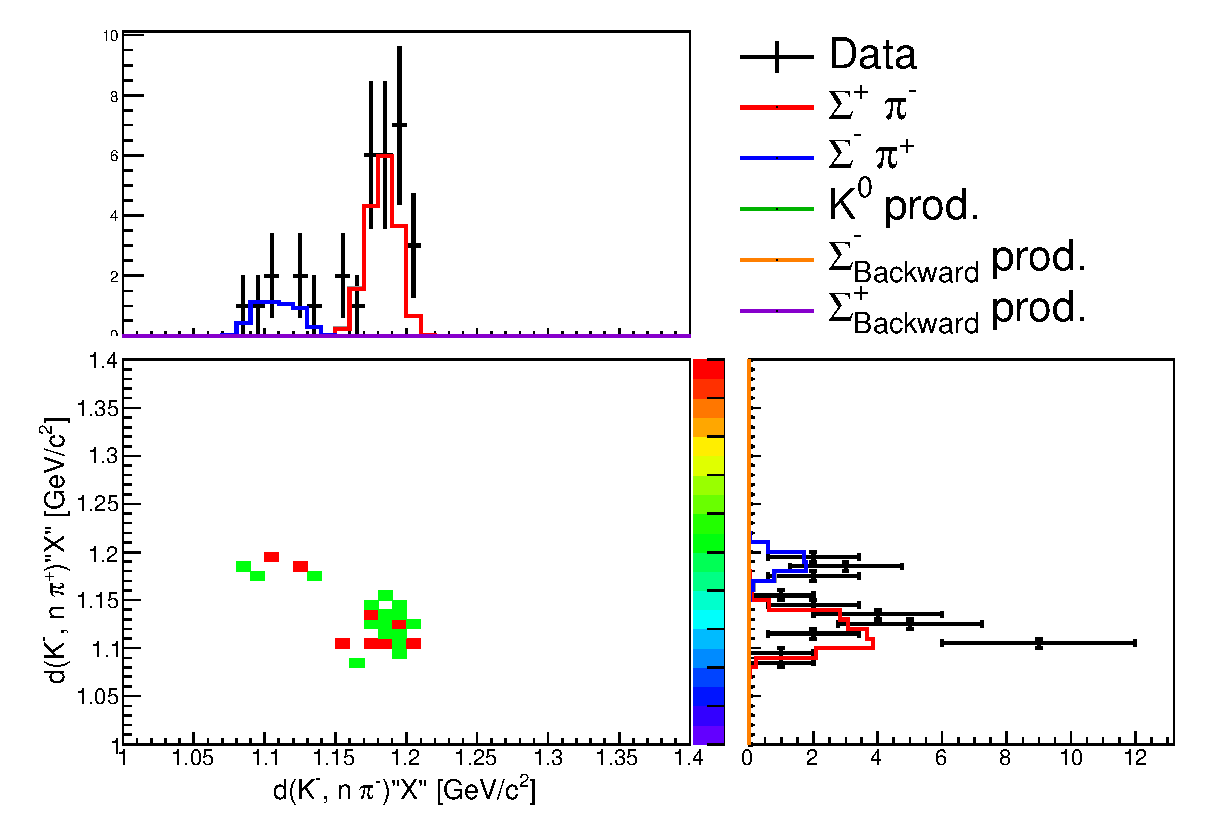
\includegraphics[width=4.3cm]{../pic/Run78/KN_ana_NC170_2sigma/KNpi_MM_1.eps}
    \end{minipage}
    \begin{minipage}{0.33\hsize}
      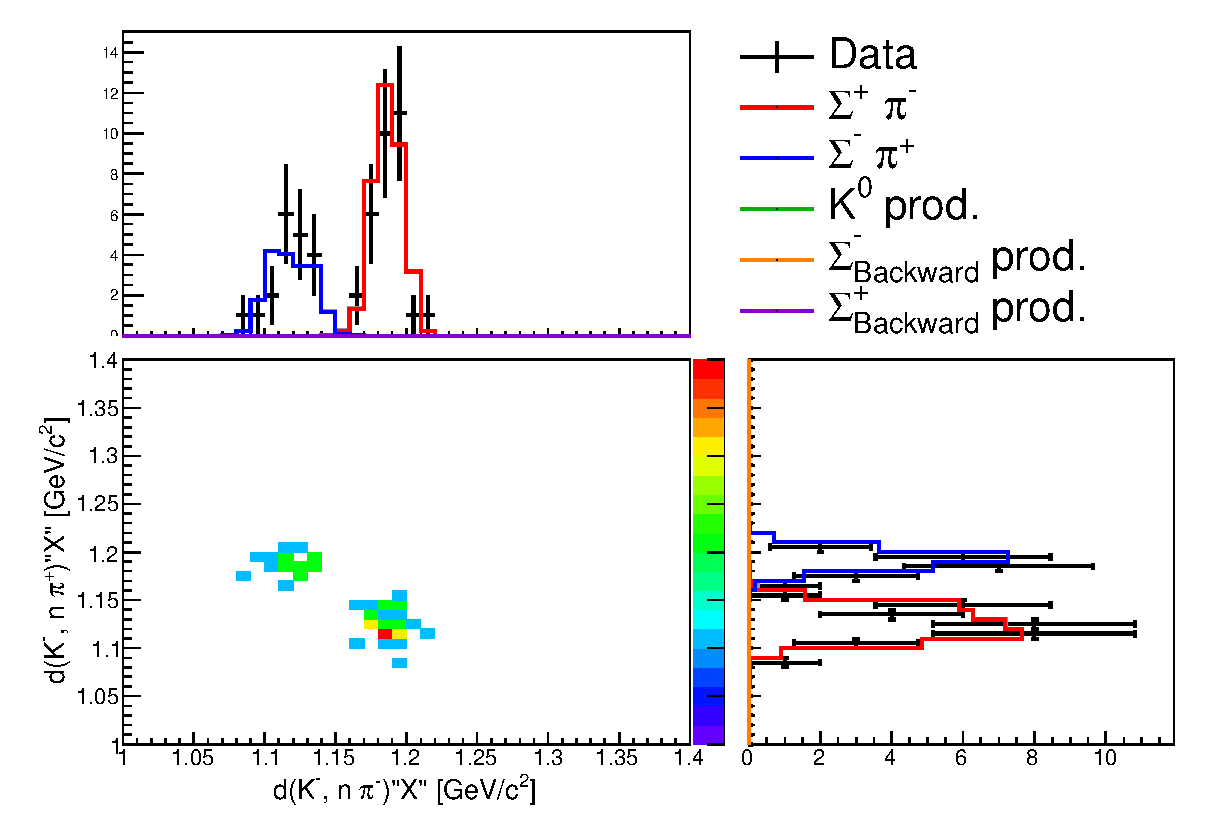
\includegraphics[width=4.3cm]{../pic/Run78/KN_ana_NC170_2sigma/KNpi_MM_2.eps}
    \end{minipage}
  \end{tabular}

  \begin{tabular}{ccc}
    \begin{minipage}{0.33\hsize}
      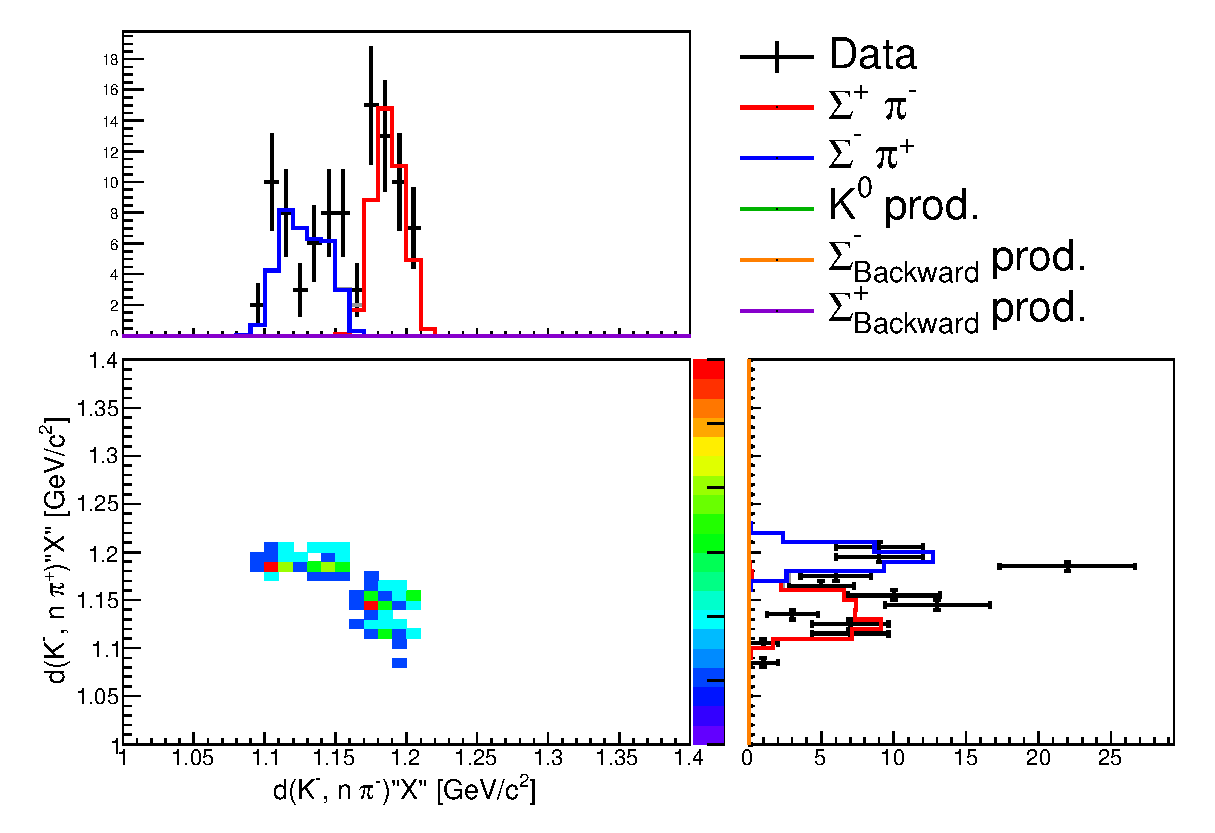
\includegraphics[width=4.3cm]{../pic/Run78/KN_ana_NC170_2sigma/KNpi_MM_3.eps}
    \end{minipage}
    \begin{minipage}{0.33\hsize}
      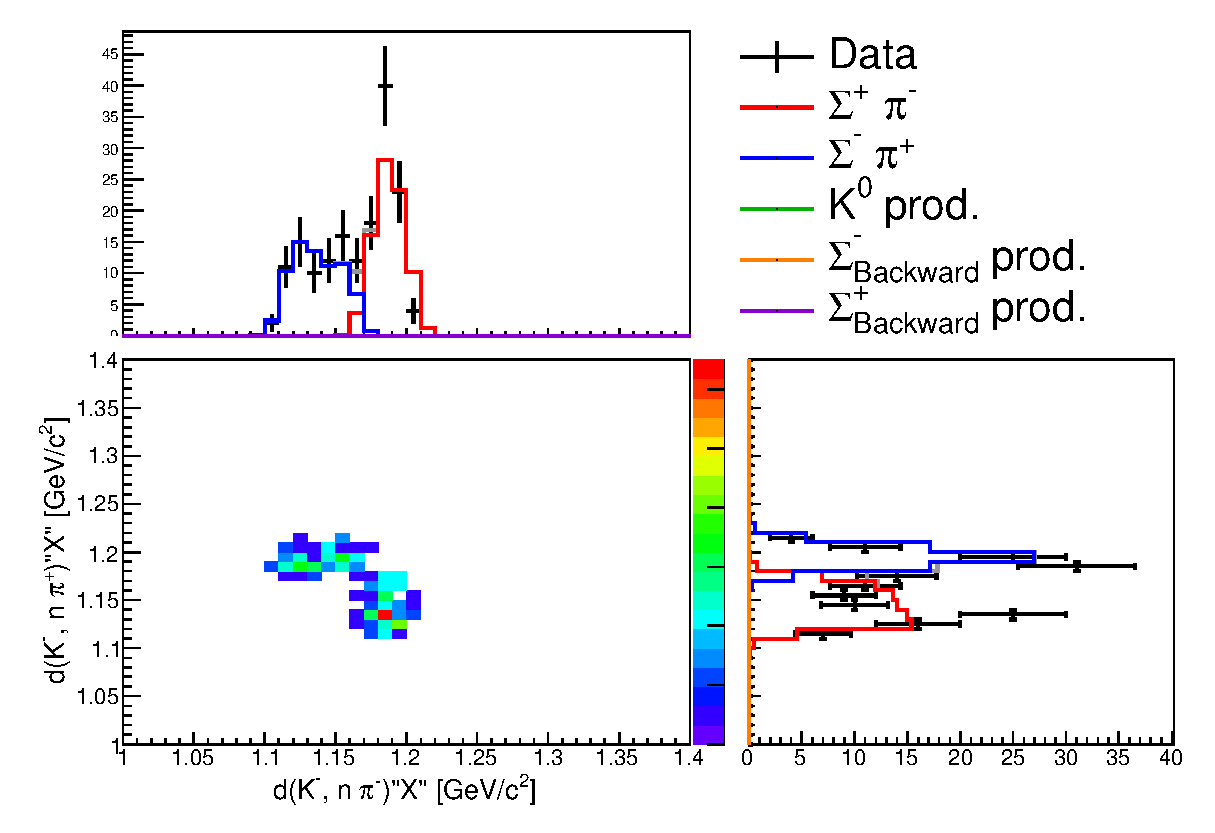
\includegraphics[width=4.3cm]{../pic/Run78/KN_ana_NC170_2sigma/KNpi_MM_4.eps}
    \end{minipage}
    \begin{minipage}{0.33\hsize}
      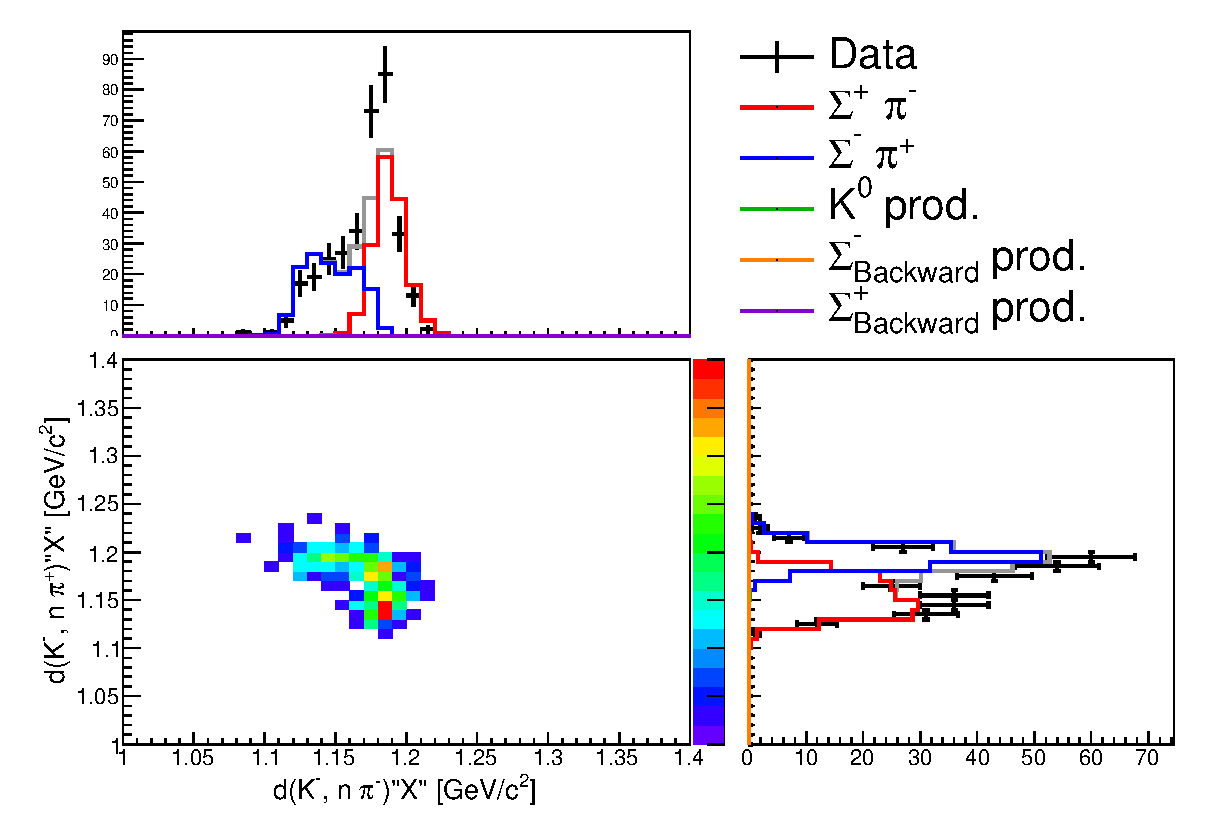
\includegraphics[width=4.3cm]{../pic/Run78/KN_ana_NC170_2sigma/KNpi_MM_5.eps}
    \end{minipage}
  \end{tabular}

  \begin{tabular}{ccc}
    \begin{minipage}{0.33\hsize}
      \includegraphics[width=4.3cm]{../pic/Run78/KN_ana_NC170_2sigma/KNpi_MM_6.eps}
    \end{minipage}
    \begin{minipage}{0.33\hsize}
      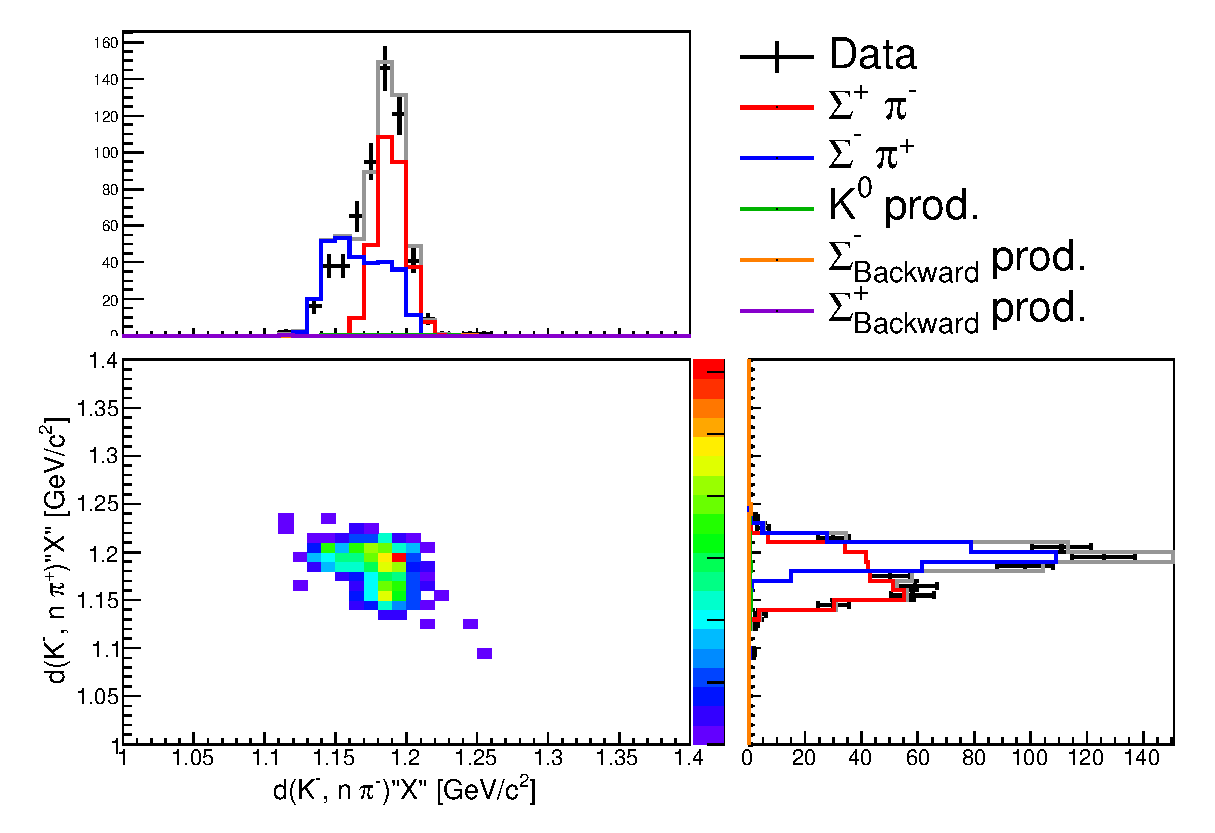
\includegraphics[width=4.3cm]{../pic/Run78/KN_ana_NC170_2sigma/KNpi_MM_7.eps}
    \end{minipage}
    \begin{minipage}{0.33\hsize}
      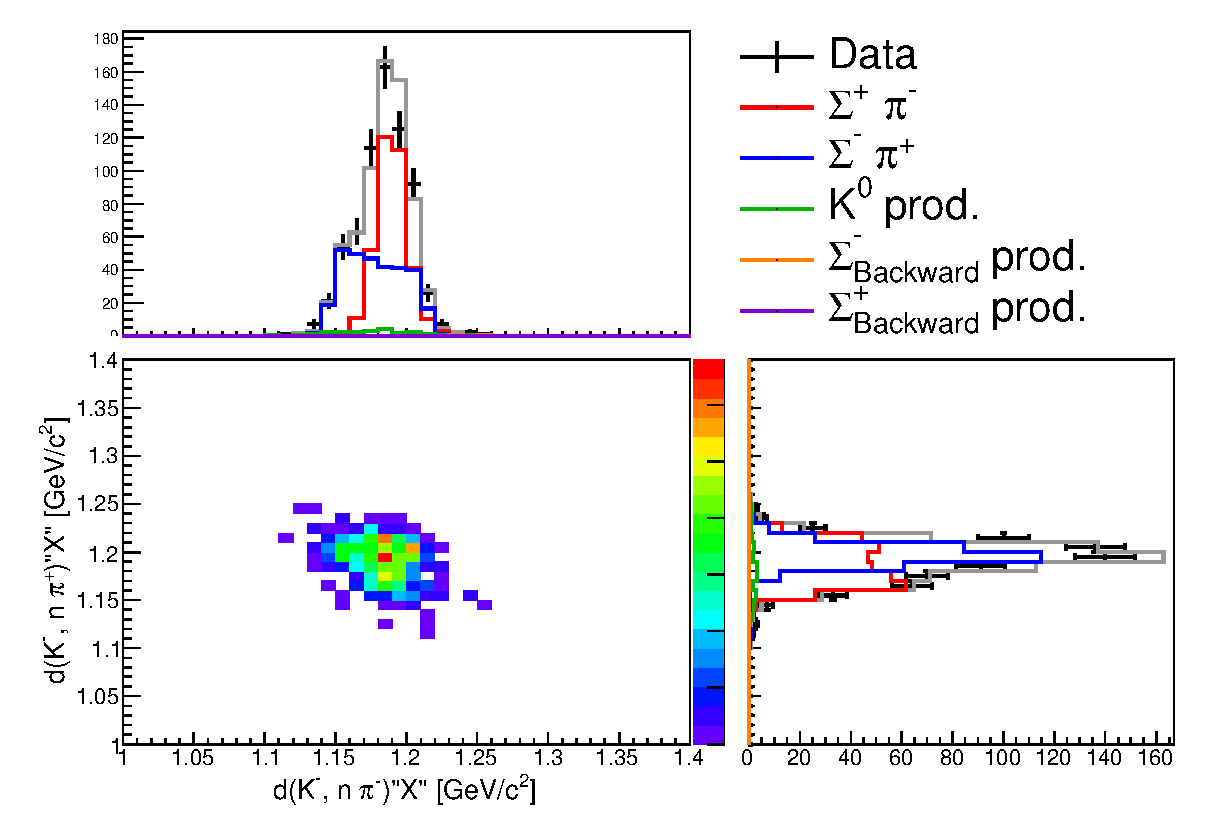
\includegraphics[width=4.3cm]{../pic/Run78/KN_ana_NC170_2sigma/KNpi_MM_8.eps}
    \end{minipage}
  \end{tabular}

  \begin{tabular}{ccc}
    \begin{minipage}{0.33\hsize}
      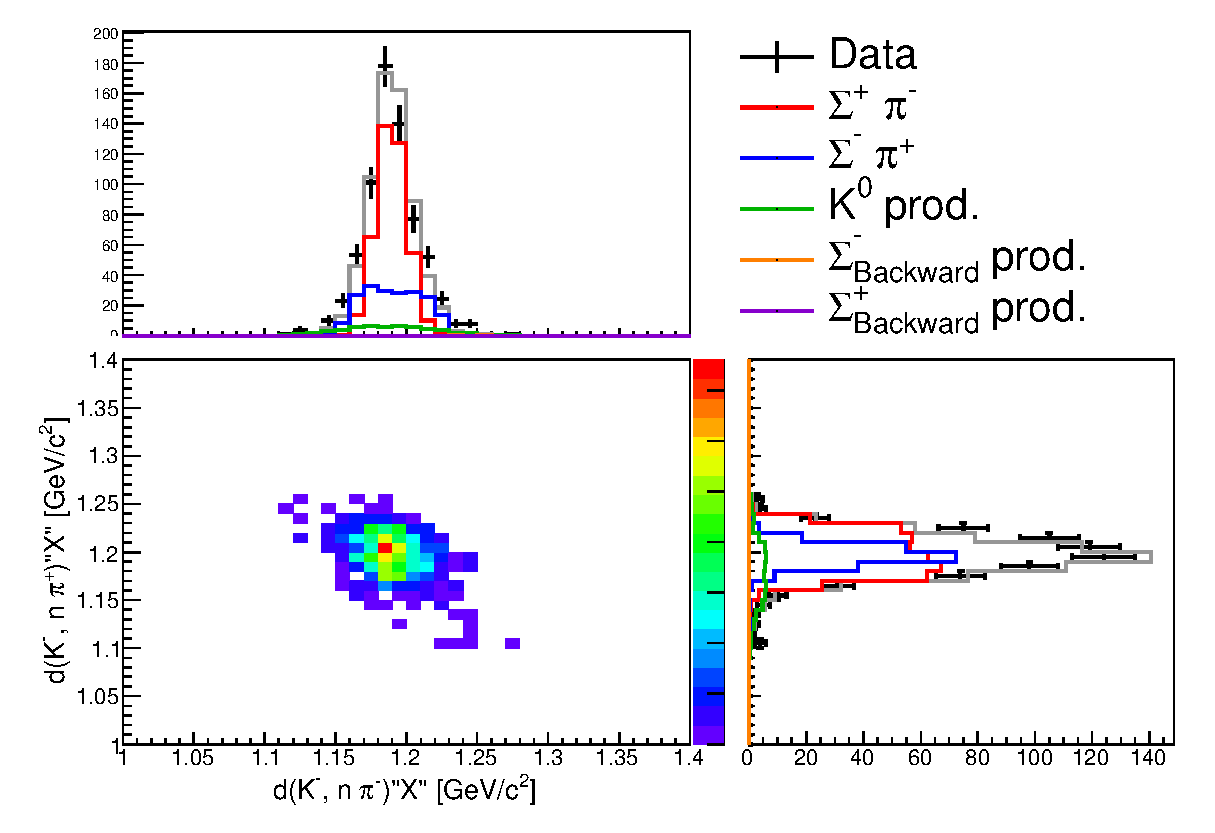
\includegraphics[width=4.3cm]{../pic/Run78/KN_ana_NC170_2sigma/KNpi_MM_9.eps}
    \end{minipage}
    \begin{minipage}{0.33\hsize}
      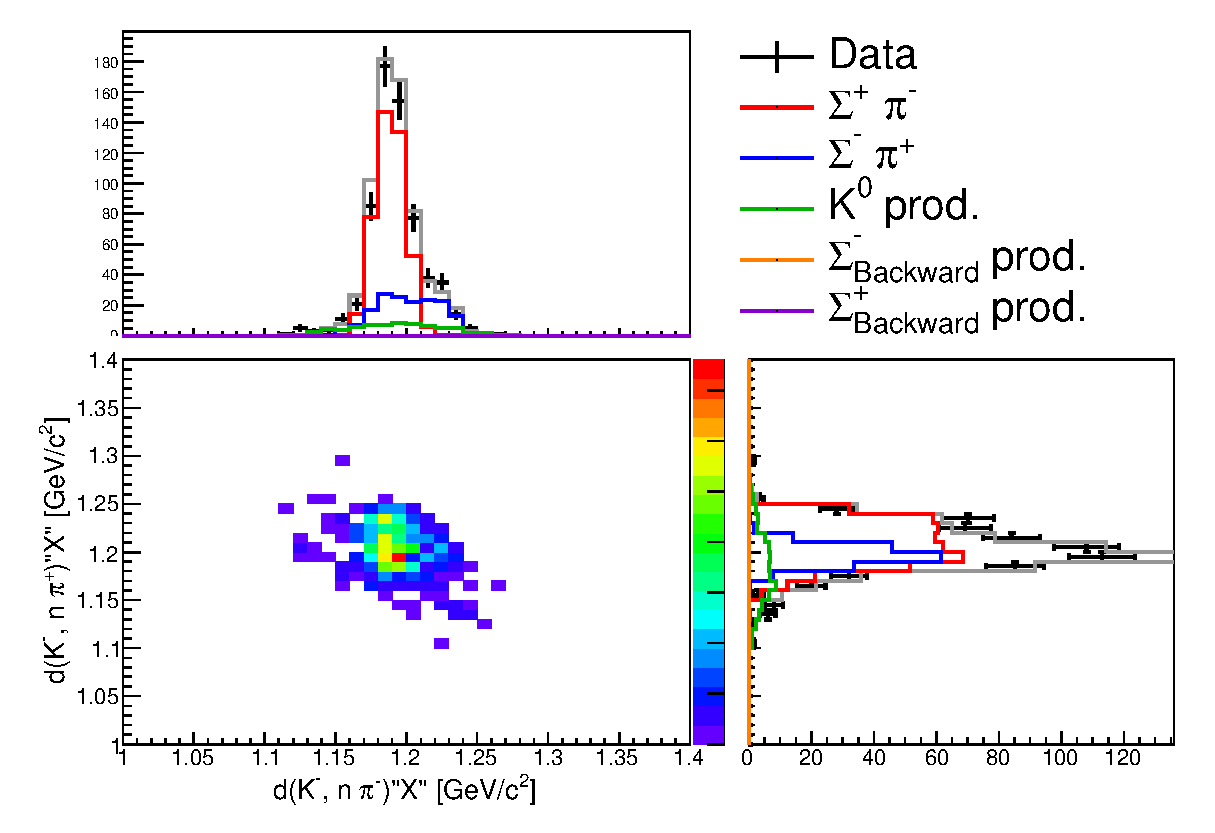
\includegraphics[width=4.3cm]{../pic/Run78/KN_ana_NC170_2sigma/KNpi_MM_10.eps}
    \end{minipage}
    \begin{minipage}{0.33\hsize}
      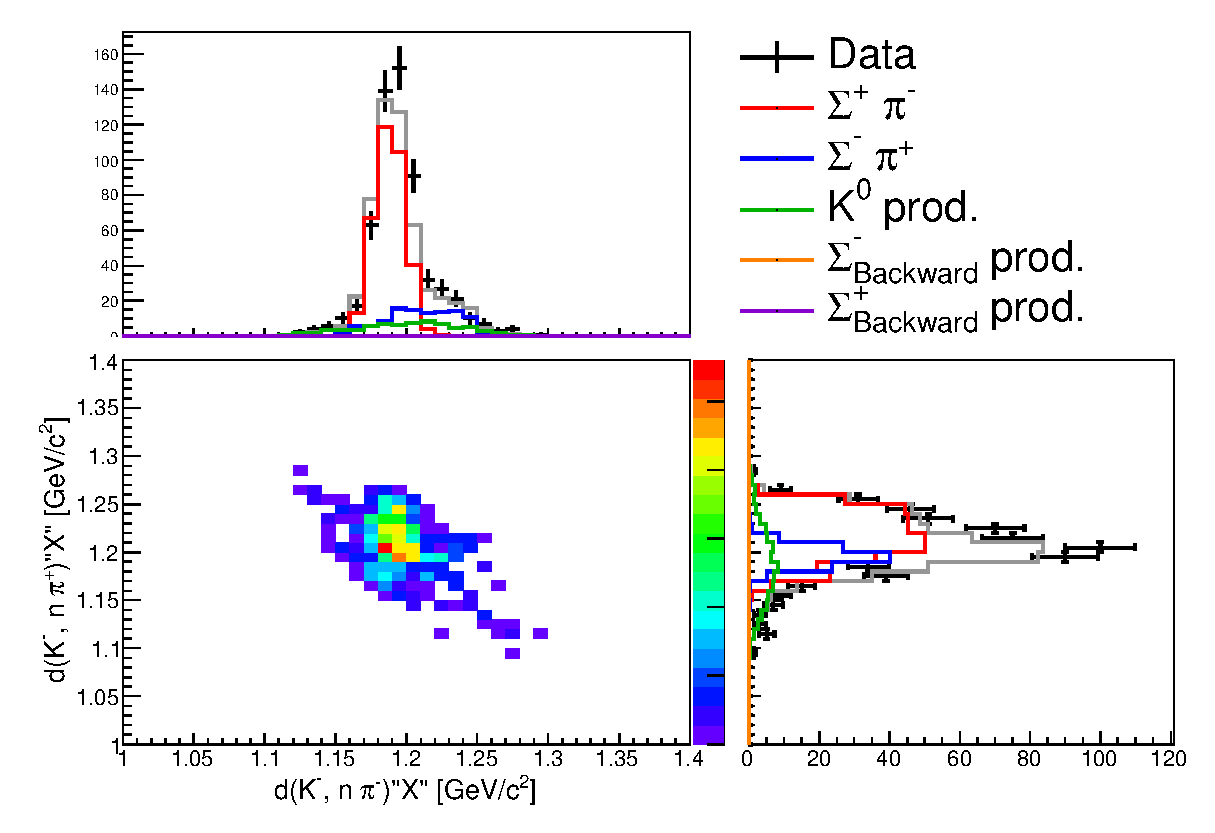
\includegraphics[width=4.3cm]{../pic/Run78/KN_ana_NC170_2sigma/KNpi_MM_11.eps}
    \end{minipage}
  \end{tabular}

  \begin{tabular}{ccc}
    \begin{minipage}{0.33\hsize}
      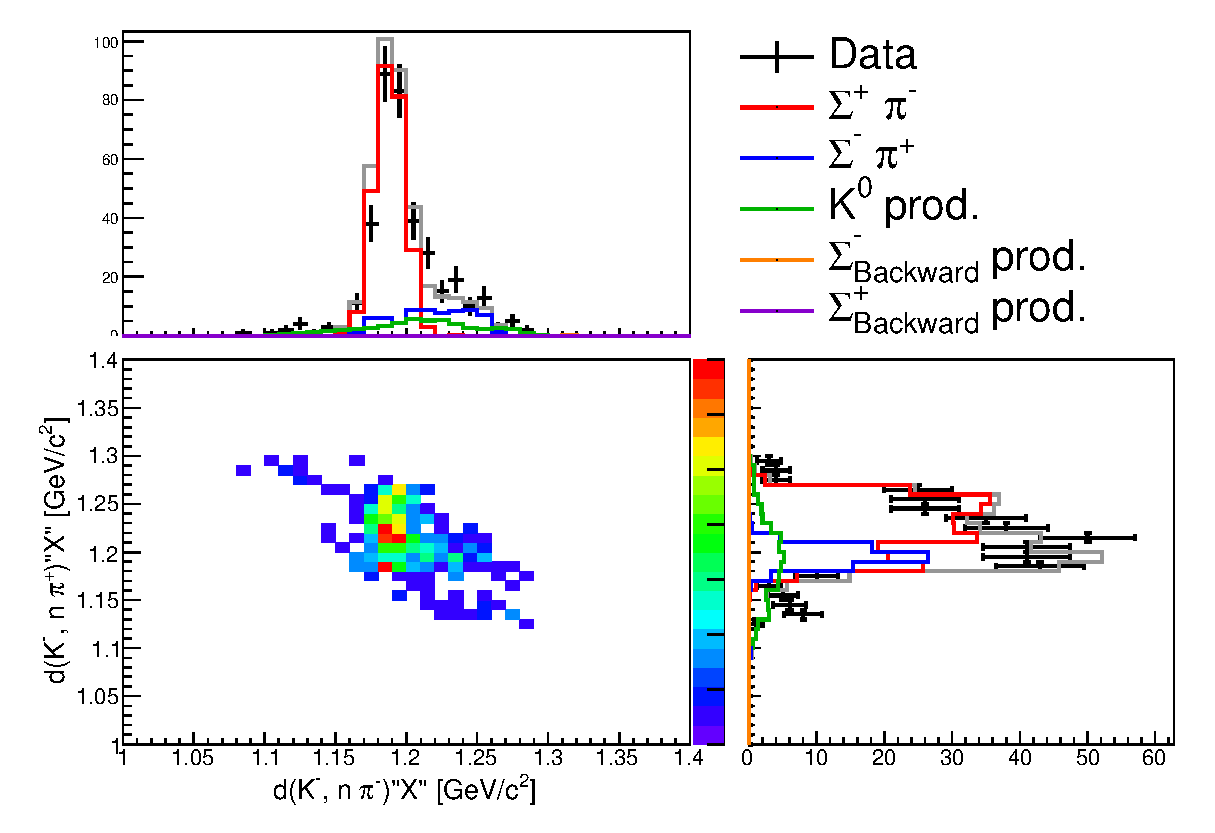
\includegraphics[width=4.3cm]{../pic/Run78/KN_ana_NC170_2sigma/KNpi_MM_12.eps}
    \end{minipage}
    \begin{minipage}{0.33\hsize}
      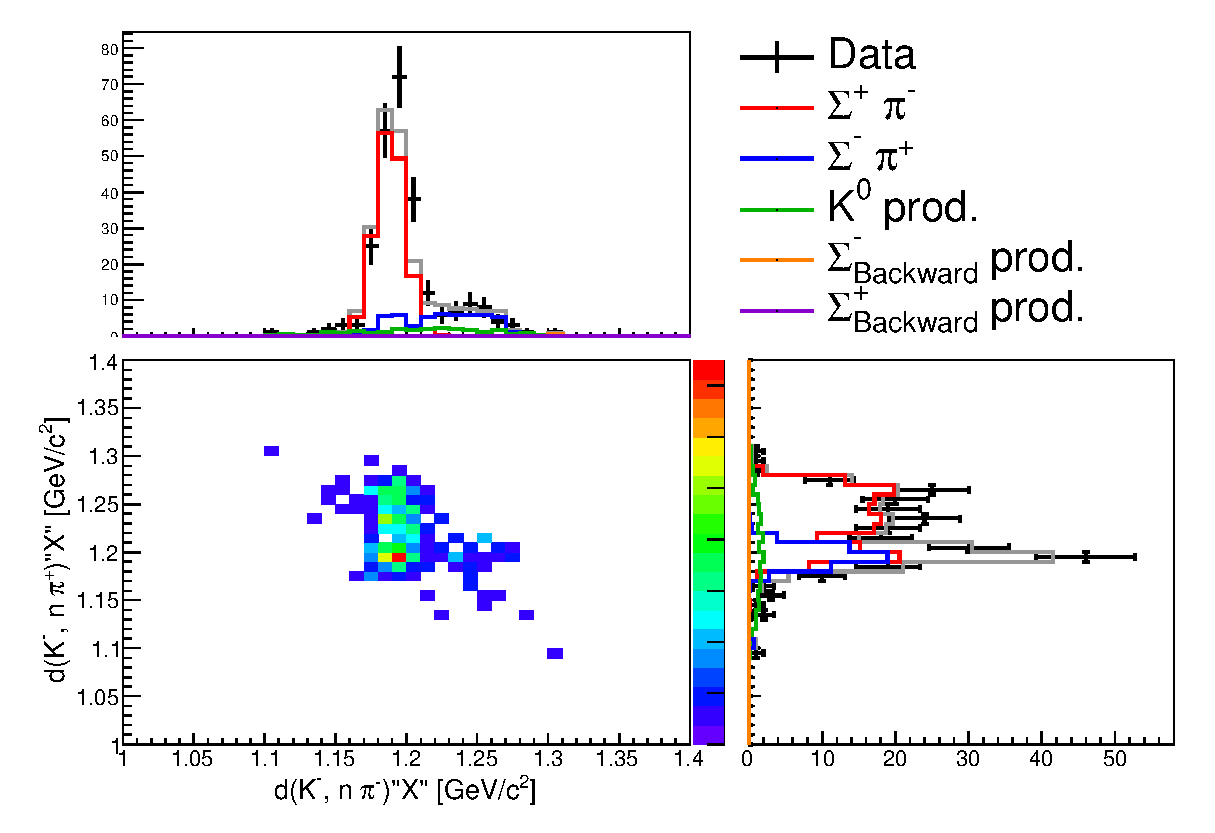
\includegraphics[width=4.3cm]{../pic/Run78/KN_ana_NC170_2sigma/KNpi_MM_13.eps}
    \end{minipage}
    \begin{minipage}{0.33\hsize}
      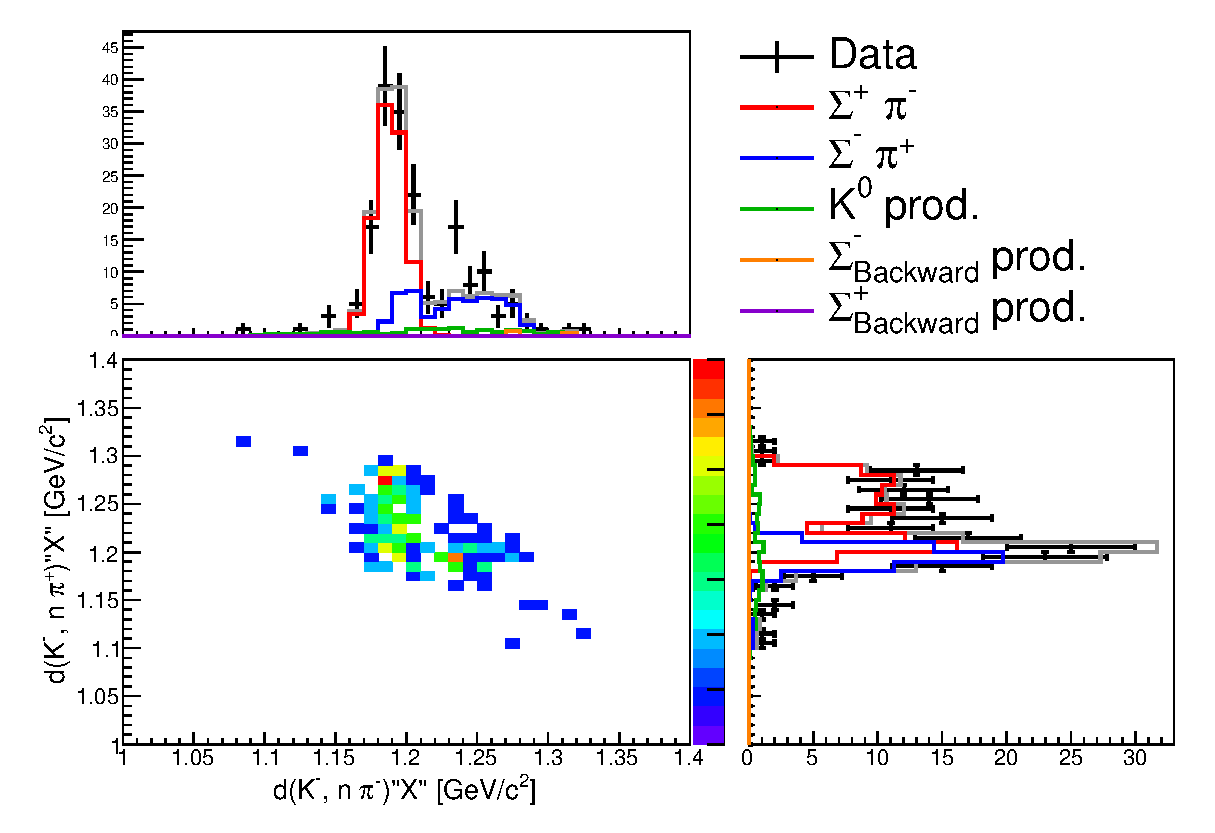
\includegraphics[width=4.3cm]{../pic/Run78/KN_ana_NC170_2sigma/KNpi_MM_14.eps}
    \end{minipage}
  \end{tabular}

  \begin{tabular}{ccc}
    \begin{minipage}{0.33\hsize}
      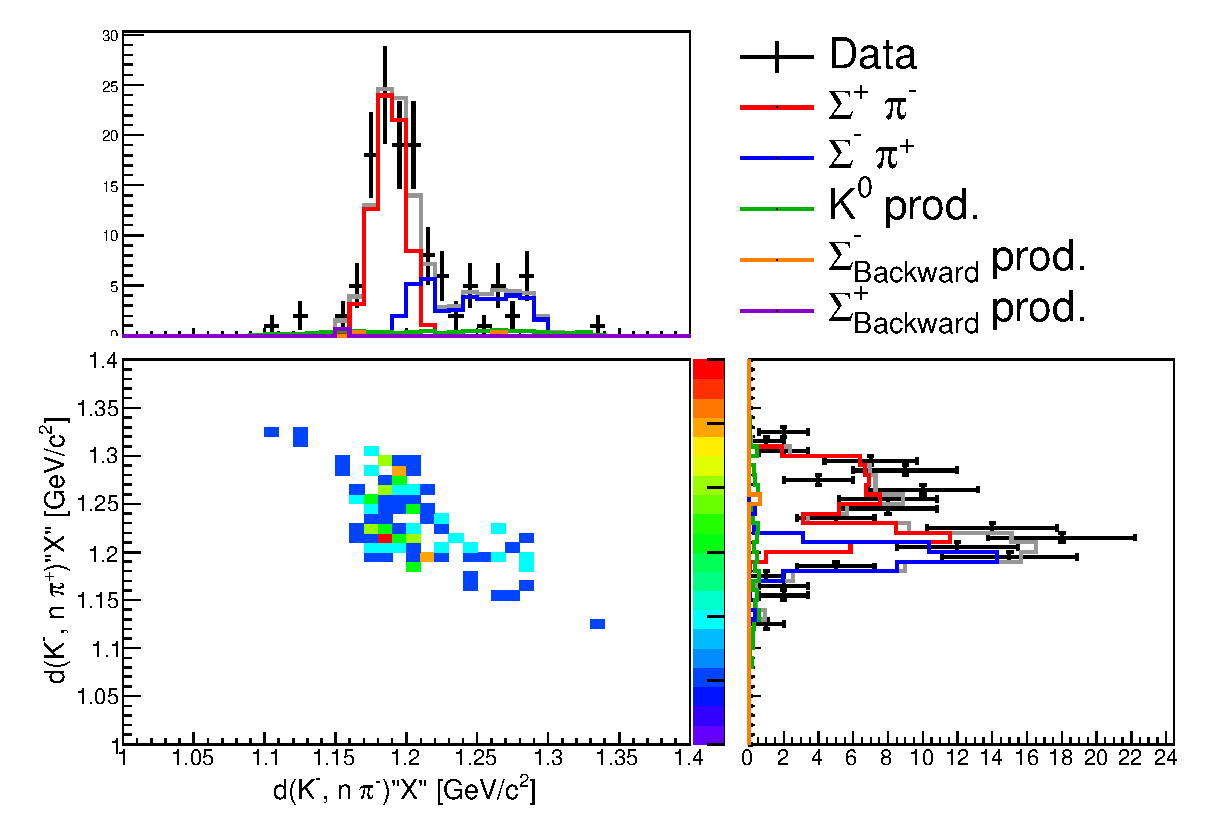
\includegraphics[width=4.3cm]{../pic/Run78/KN_ana_NC170_2sigma/KNpi_MM_15.eps}
    \end{minipage}
    \begin{minipage}{0.33\hsize}
      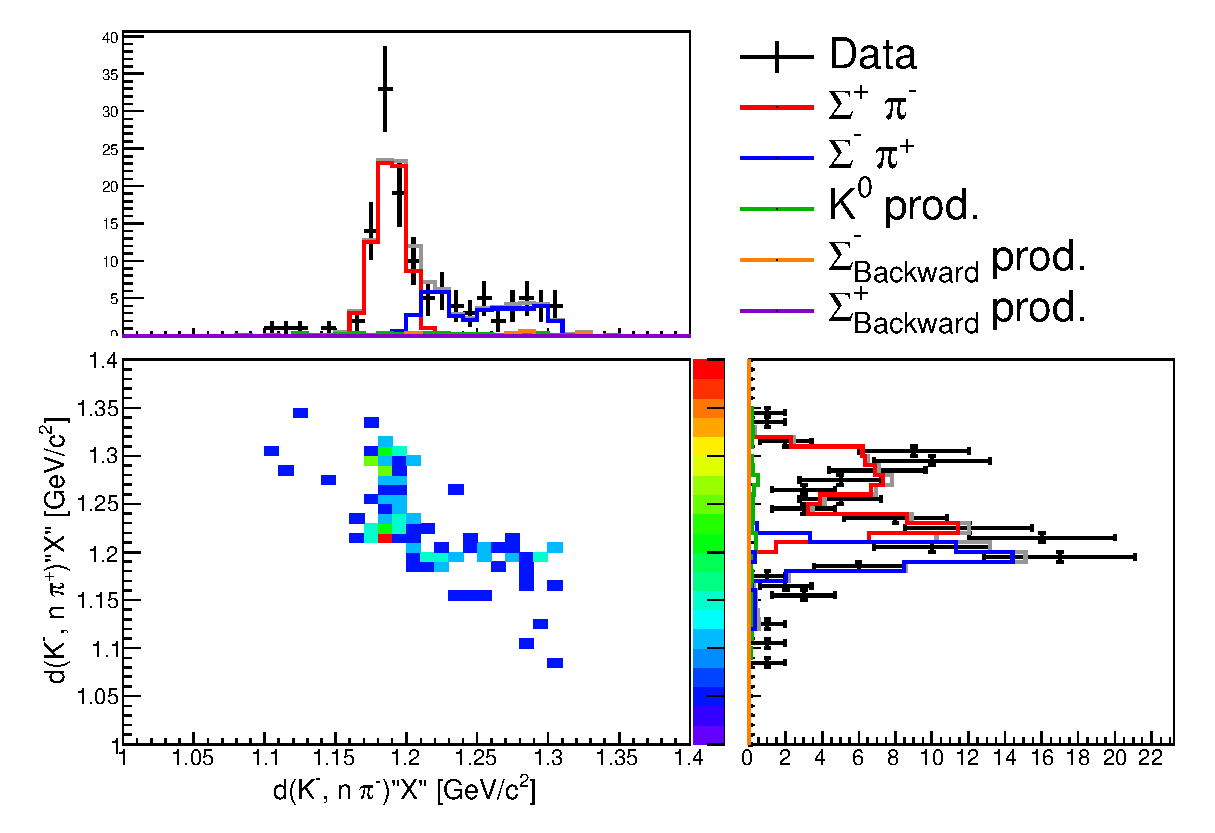
\includegraphics[width=4.3cm]{../pic/Run78/KN_ana_NC170_2sigma/KNpi_MM_16.eps}
    \end{minipage}
    \begin{minipage}{0.33\hsize}
      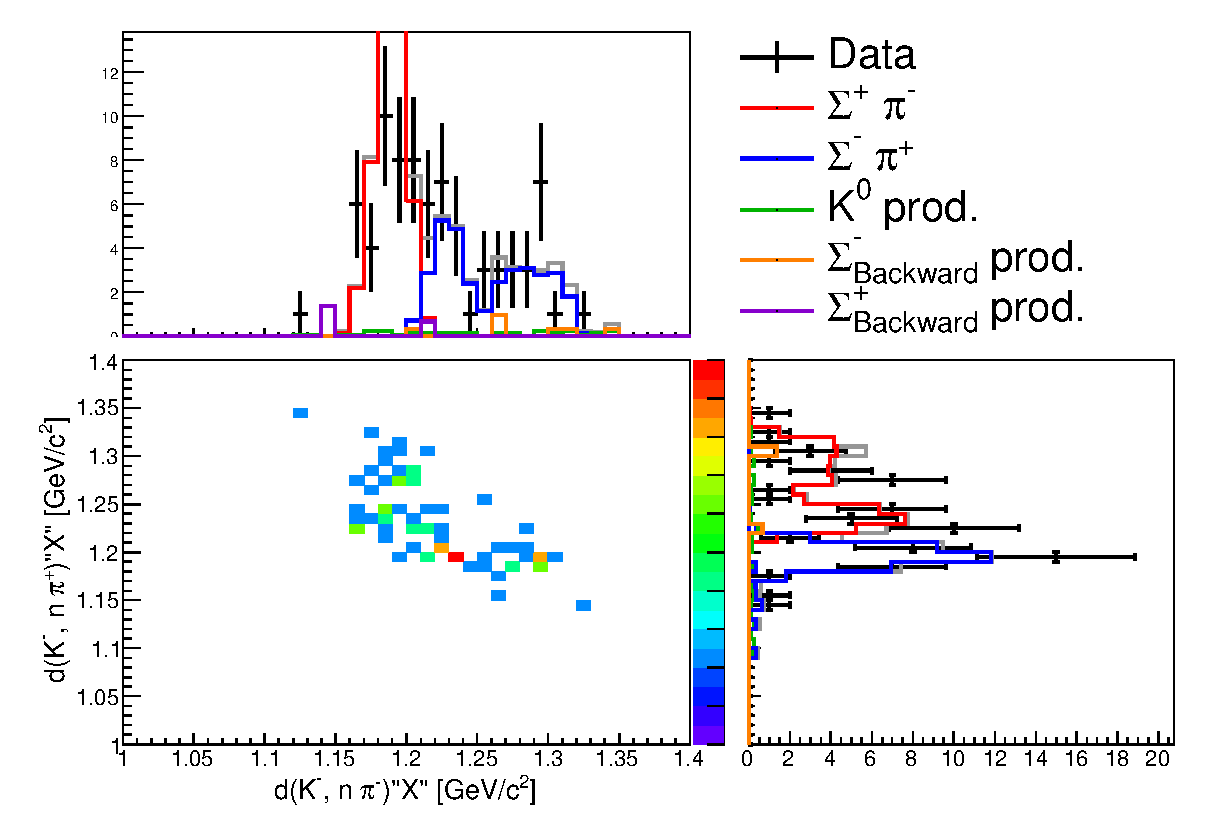
\includegraphics[width=4.3cm]{../pic/Run78/KN_ana_NC170_2sigma/KNpi_MM_17.eps}
    \end{minipage}
  \end{tabular}
\end{figure}

\begin{figure}
  \begin{tabular}{ccc}
    \begin{minipage}{0.33\hsize}
      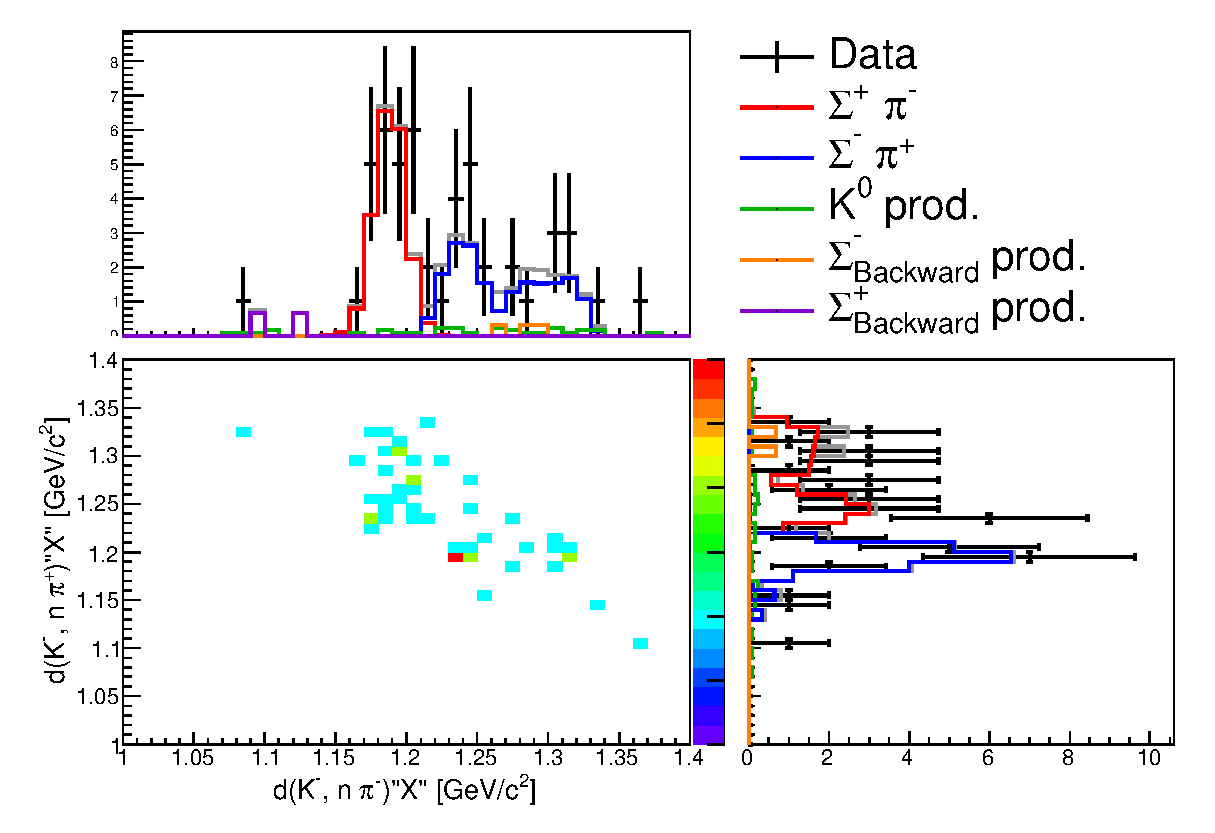
\includegraphics[width=4.3cm]{../pic/Run78/KN_ana_NC170_2sigma/KNpi_MM_18.eps}
    \end{minipage}
    \begin{minipage}{0.33\hsize}
      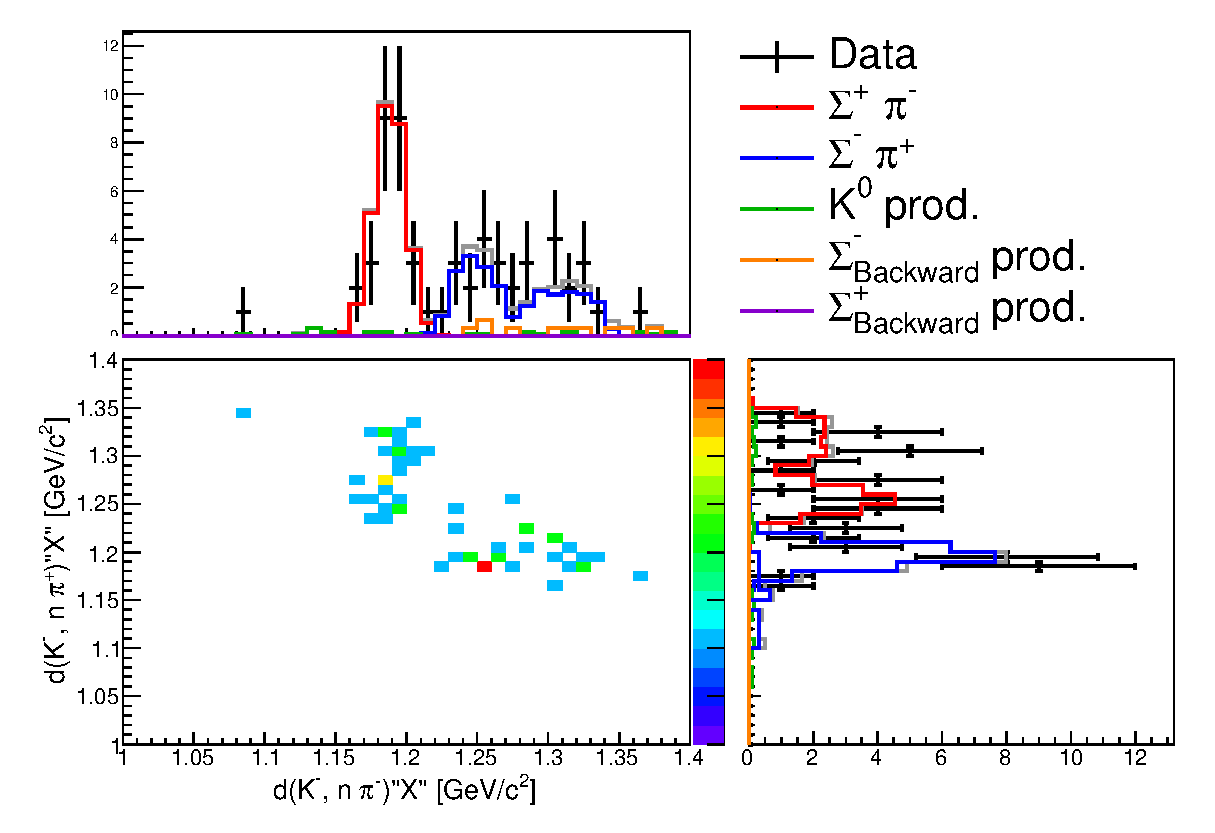
\includegraphics[width=4.3cm]{../pic/Run78/KN_ana_NC170_2sigma/KNpi_MM_19.eps}
    \end{minipage}
    \begin{minipage}{0.33\hsize}
      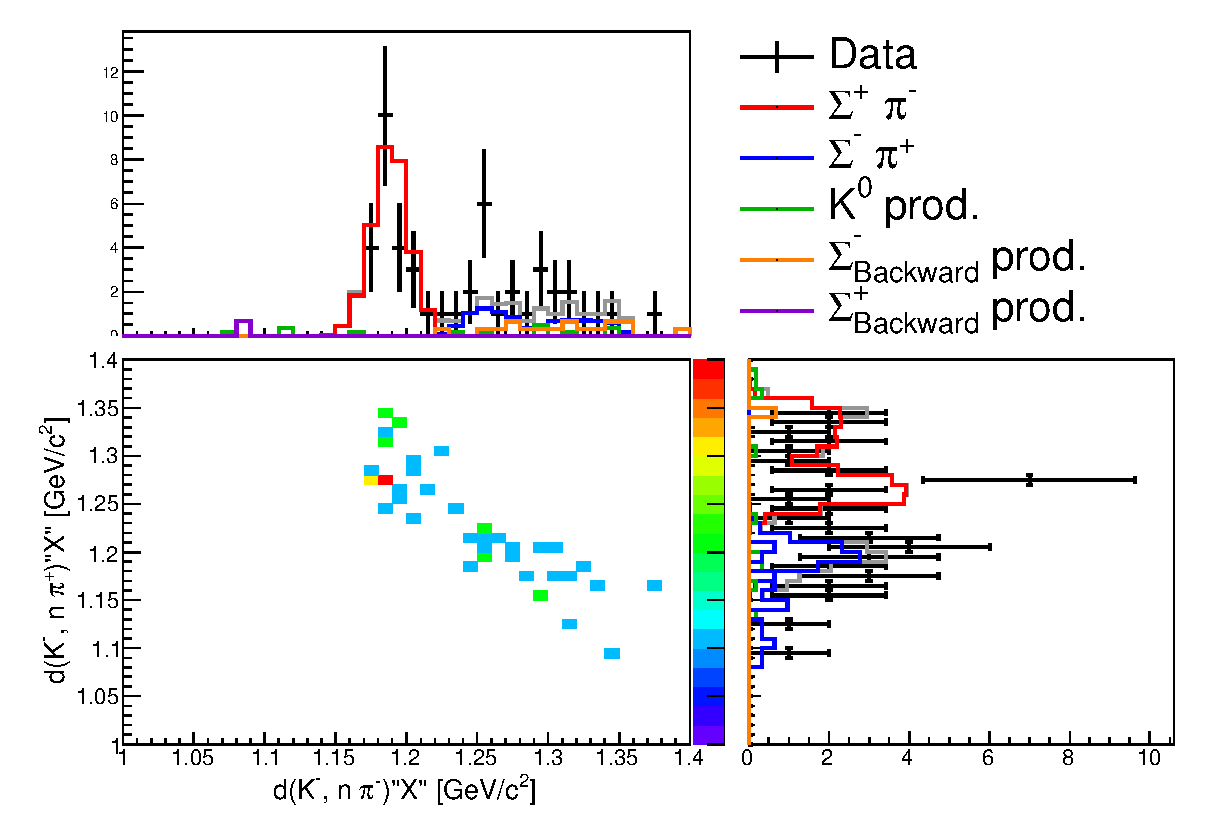
\includegraphics[width=4.3cm]{../pic/Run78/KN_ana_NC170_2sigma/KNpi_MM_20.eps}
    \end{minipage}
  \end{tabular}

  \begin{tabular}{ccc}
    \begin{minipage}{0.33\hsize}
      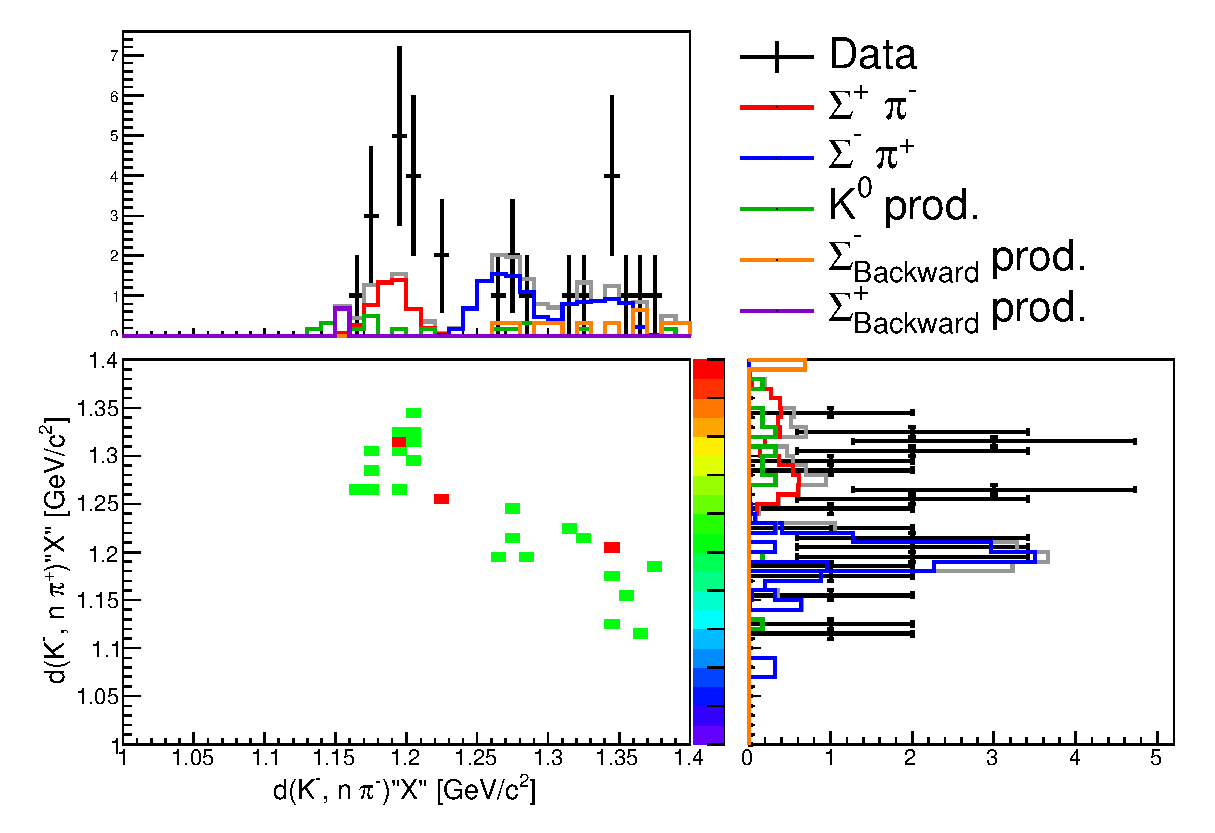
\includegraphics[width=4.3cm]{../pic/Run78/KN_ana_NC170_2sigma/KNpi_MM_21.eps}
    \end{minipage}
    \begin{minipage}{0.33\hsize}
      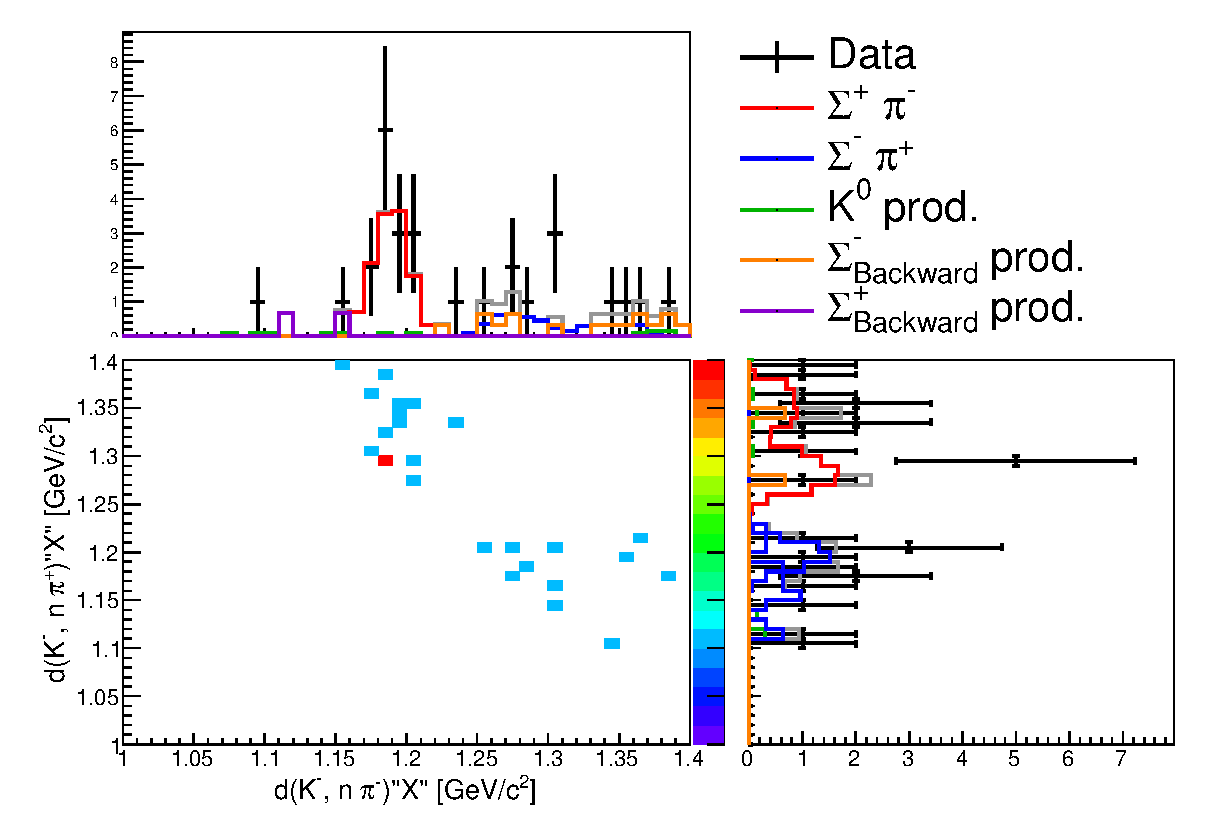
\includegraphics[width=4.3cm]{../pic/Run78/KN_ana_NC170_2sigma/KNpi_MM_22.eps}
    \end{minipage}
    \begin{minipage}{0.33\hsize}
      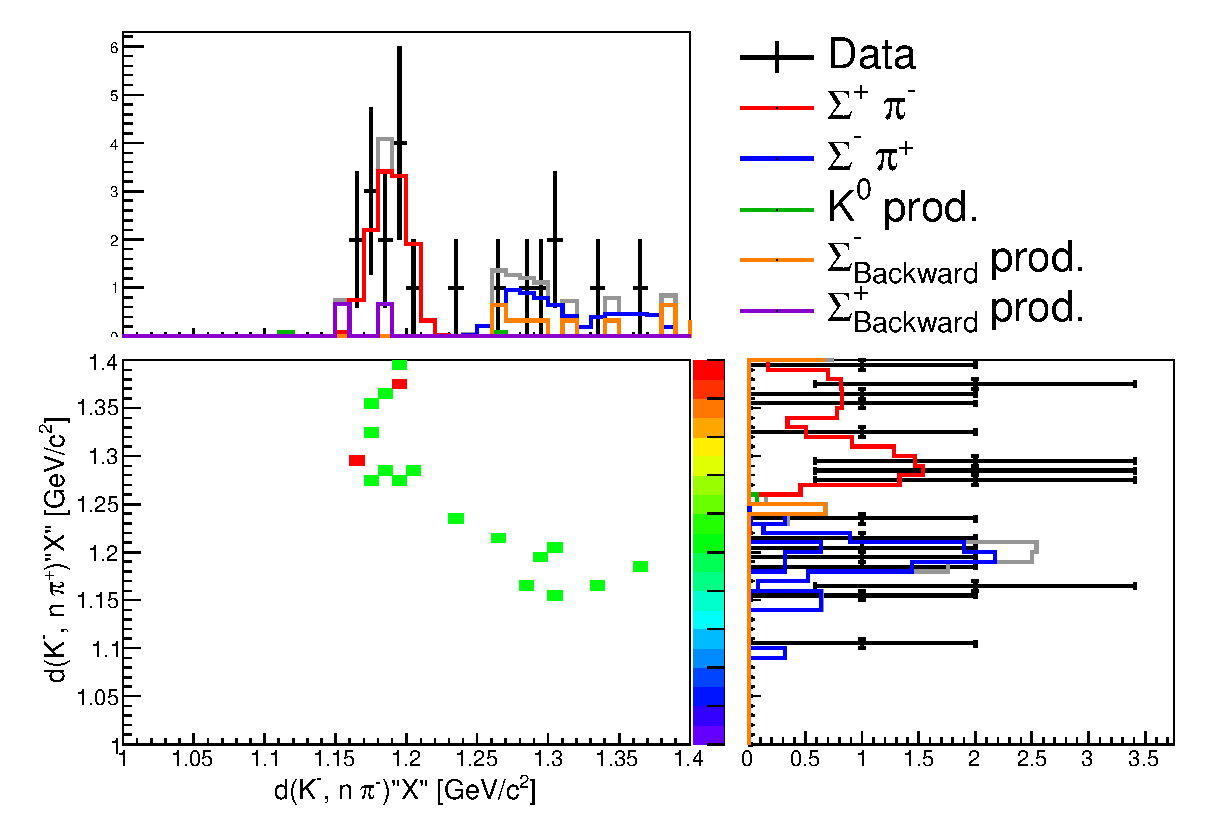
\includegraphics[width=4.3cm]{../pic/Run78/KN_ana_NC170_2sigma/KNpi_MM_23.eps}
    \end{minipage}
  \end{tabular}

  \begin{tabular}{ccc}
    \begin{minipage}{0.33\hsize}
      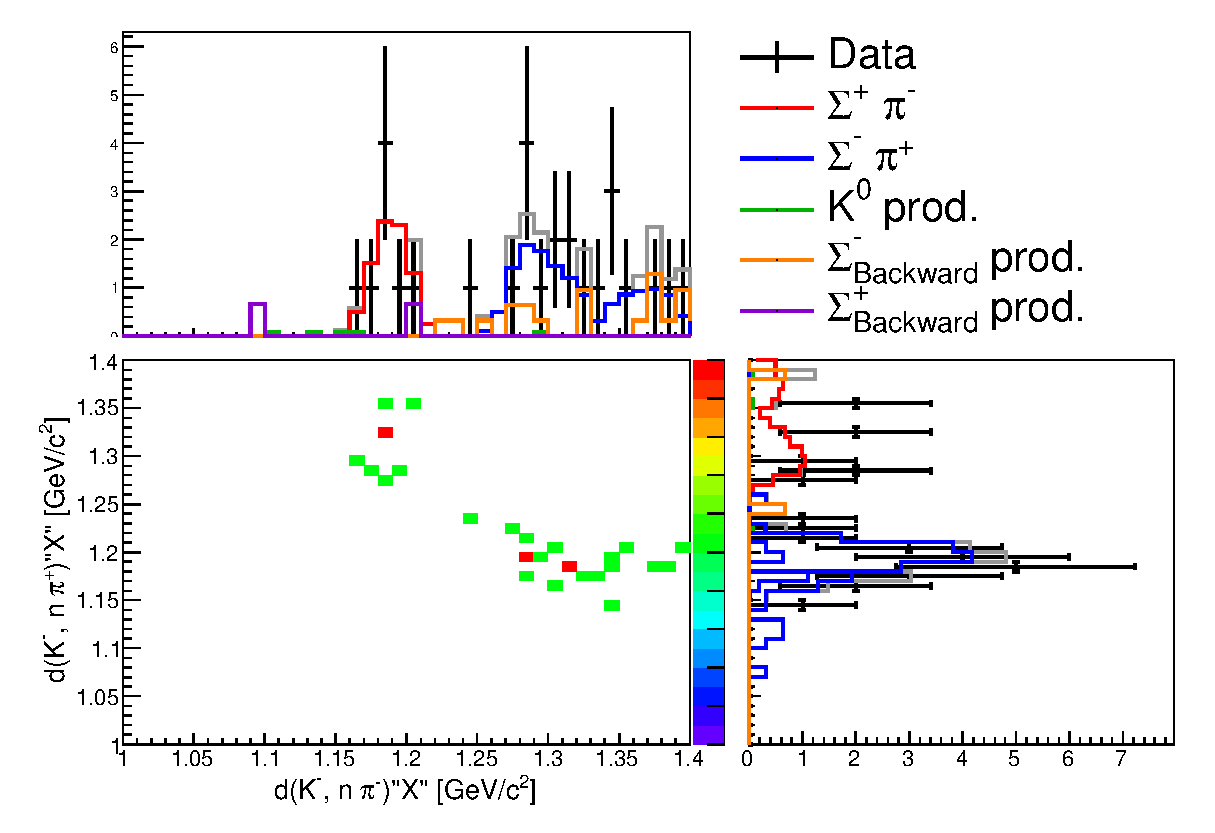
\includegraphics[width=4.3cm]{../pic/Run78/KN_ana_NC170_2sigma/KNpi_MM_24.eps}
    \end{minipage}
    \begin{minipage}{0.33\hsize}
    \end{minipage}
    \begin{minipage}{0.33\hsize}
    \end{minipage}
  \end{tabular}
  
  \caption{
    These figures are shown separately for each bin of $d(K^-, n)$ for fitting to separate $\pi^- \Sigma^+$ and $\pi^+ \Sigma^-$ modes.
    The top left panel corresponds to the lowest missing mass bin ($1.35$-$1.36$GeV),
    and each subsequent bin is shown to the right.
    That is, each row represents a 0.03 GeV range, covering the overall range from 1.35 to 1.60 GeV.
  }
  \label{fig:fit_KNpi_MM}
\end{figure}
